\documentclass[tikz,border=6pt]{standalone}
\usepackage{xcolor}
\begin{document}
% Canonical ch-diagram for 9_1^0,1
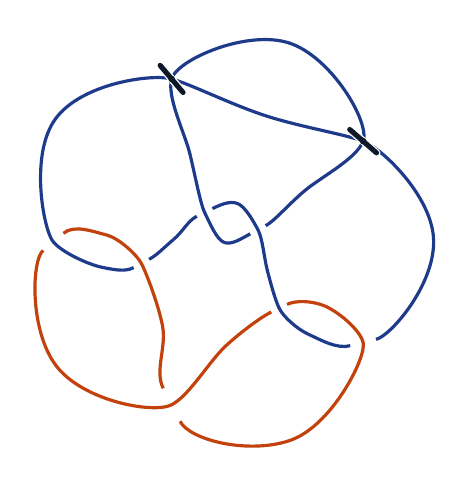
\begin{tikzpicture}[line join=round]
  \definecolor{skcomp0}{RGB}{30,58,138}
  \definecolor{skcomp1}{RGB}{194,65,12}
  \definecolor{skmark}{RGB}{15,23,42}
  \draw[skcomp0, line width=1.15pt, line cap=butt] (-1.2424,-0.3268) .. controls (-1.3468,-0.3828) and (-1.4828,-0.3562) .. (-1.6498,-0.3216);
  \draw[skcomp1, line width=1.15pt, line cap=butt] (-0.8666,-1.8599) .. controls (-0.9798,-1.6376) and (-0.8219,-1.3380) .. (-0.8762,-1.0632);
  \draw[skcomp0, line width=1.15pt, line cap=butt] (-1.0458,-0.2214) .. controls (-0.9391,-0.1641) and (-0.8538,-0.0679) .. (-0.7368,0.0289);
  \draw[skcomp0, line width=1.15pt, line cap=butt] (-0.4404,0.3247) .. controls (-0.5524,0.2697) and (-0.6197,0.1257) .. (-0.7368,0.0289);
  \draw[skcomp1, line width=1.15pt, line cap=butt] (-2.1346,0.1088) .. controls (-1.9979,0.2244) and (-1.7528,0.1294) .. (-1.5887,0.0877);
  \draw[skcomp1, line width=1.15pt, line cap=butt] (-2.3919,-0.1088) .. controls (-2.5367,-0.2312) and (-2.5679,-1.1042) .. (-2.2361,-1.5609);
  \draw[skcomp1, line width=1.15pt, line cap=butt] (-0.6534,-2.2783) .. controls (-0.5335,-2.5137) and (0.1961,-2.7000) .. (0.7329,-2.5256);
  \draw[skcomp1, line width=1.15pt, line cap=butt] (0.5054,-0.8912) .. controls (0.3924,-0.9458) and (0.1308,-1.1333) .. (-0.0747,-1.3236);
  \draw[skcomp0, line width=1.15pt, line cap=butt] (0.2385,0.1017) .. controls (0.1282,0.0433) and (0.0075,-0.0404) .. (-0.0905,-0.0085);
  \draw[skcomp0, line width=1.15pt, line cap=butt] (-0.2411,0.4225) .. controls (-0.1353,0.4744) and (-0.0271,0.5214) .. (0.0713,0.4894);
  \draw[skcomp0, line width=1.15pt, line cap=butt] (0.4347,0.2054) .. controls (0.5451,0.2637) and (0.7198,0.4715) .. (0.9272,0.6470);
  \draw[skcomp0, line width=1.15pt, line cap=butt] (1.8360,-1.2386) .. controls (2.0201,-1.1935) and (2.5679,-0.5645) .. (2.5679,0.0000);
  \draw[skcomp1, line width=1.15pt, line cap=butt] (0.7063,-0.7941) .. controls (0.8192,-0.7395) and (1.0209,-0.7486) .. (1.1782,-0.8113);
  \draw[skcomp0, line width=1.15pt, line cap=butt] (1.5087,-1.3189) .. controls (1.3334,-1.3619) and (1.1423,-1.2485) .. (0.9870,-1.1783);
  \draw[skcomp0, line width=1.15pt, line cap=round] (-2.2633,0.0000) .. controls (-2.1467,-0.1378) and (-1.8167,-0.2871) .. (-1.6498,-0.3216);
  \draw[skcomp1, line width=1.15pt, line cap=round] (-1.1441,-0.2741) .. controls (-1.0847,-0.3847) and (-0.9306,-0.7884) .. (-0.8762,-1.0632);
  \draw[skcomp1, line width=1.15pt, line cap=round] (-1.1441,-0.2741) .. controls (-1.2034,-0.1635) and (-1.4246,0.0460) .. (-1.5887,0.0877);
  \draw[skcomp0, line width=1.15pt, line cap=round] (-2.2633,0.0000) .. controls (-2.3857,0.1448) and (-2.5679,1.1042) .. (-2.2361,1.5609);
  \draw[skcomp0, line width=1.15pt, line cap=round] (-0.7600,2.0691) .. controls (-1.0048,2.1366) and (-1.9043,2.0175) .. (-2.2361,1.5609);
  \draw[skcomp1, line width=1.15pt, line cap=round] (-0.7600,-2.0691) .. controls (-0.9953,-2.1890) and (-1.9043,-2.0175) .. (-2.2361,-1.5609);
  \draw[skcomp1, line width=1.15pt, line cap=round] (1.6724,-1.2788) .. controls (1.7176,-1.4629) and (1.2697,-2.3511) .. (0.7329,-2.5256);
  \draw[skcomp1, line width=1.15pt, line cap=round] (-0.7600,-2.0691) .. controls (-0.5377,-1.9558) and (-0.2802,-1.5140) .. (-0.0747,-1.3236);
  \draw[skcomp0, line width=1.15pt, line cap=round] (-0.3407,0.3736) .. controls (-0.2857,0.2616) and (-0.1884,0.0233) .. (-0.0905,-0.0085);
  \draw[skcomp0, line width=1.15pt, line cap=round] (0.3366,0.1535) .. controls (0.2815,0.2578) and (0.1697,0.4574) .. (0.0713,0.4894);
  \draw[skcomp0, line width=1.15pt, line cap=round] (-0.3407,0.3736) .. controls (-0.3957,0.4857) and (-0.4638,0.8561) .. (-0.5285,1.1199);
  \draw[skcomp0, line width=1.15pt, line cap=round] (-0.7600,2.0691) .. controls (-0.8237,1.8379) and (-0.5931,1.3837) .. (-0.5285,1.1199);
  \draw[skcomp0, line width=1.15pt, line cap=round] (-0.7600,2.0691) .. controls (-0.5152,2.0016) and (-0.0031,1.7438) .. (0.4329,1.6021);
  \draw[skcomp0, line width=1.15pt, line cap=round] (1.6724,1.2788) .. controls (1.4347,1.3681) and (0.8689,1.4605) .. (0.4329,1.6021);
  \draw[skcomp0, line width=1.15pt, line cap=round] (-0.7600,2.0691) .. controls (-0.6925,2.3139) and (0.1961,2.7000) .. (0.7329,2.5256);
  \draw[skcomp0, line width=1.15pt, line cap=round] (1.6724,1.2788) .. controls (1.7617,1.5165) and (1.2697,2.3511) .. (0.7329,2.5256);
  \draw[skcomp0, line width=1.15pt, line cap=round] (1.6724,1.2788) .. controls (1.5880,1.0543) and (1.1346,0.8224) .. (0.9272,0.6470);
  \draw[skcomp0, line width=1.15pt, line cap=round] (1.6724,1.2788) .. controls (1.9101,1.1895) and (2.5679,0.5645) .. (2.5679,0.0000);
  \draw[skcomp1, line width=1.15pt, line cap=round] (1.6724,-1.2788) .. controls (1.6297,-1.1049) and (1.3355,-0.8741) .. (1.1782,-0.8113);
  \draw[skcomp0, line width=1.15pt, line cap=round] (0.6058,-0.8427) .. controls (0.6574,-0.9494) and (0.8317,-1.1082) .. (0.9870,-1.1783);
  \draw[skcomp0, line width=1.15pt, line cap=round] (0.6058,-0.8427) .. controls (0.5531,-0.7337) and (0.4922,-0.5052) .. (0.4544,-0.3581);
  \draw[skcomp0, line width=1.15pt, line cap=round] (0.3366,0.1535) .. controls (0.3950,0.0432) and (0.4166,-0.2110) .. (0.4544,-0.3581);
  \draw[white, line width=2.8pt, line cap=round] (-0.9057,2.2415) -- (-0.6143,1.8967);
  \draw[skmark, line width=1.85pt, line cap=round] (-0.9057,2.2415) -- (-0.6143,1.8967);
  \fill[skmark] (-0.7600,2.0691) circle (1.2pt);
  \draw[white, line width=2.8pt, line cap=round] (1.8425,1.1304) -- (1.5022,1.4271);
  \draw[skmark, line width=1.85pt, line cap=round] (1.8425,1.1304) -- (1.5022,1.4271);
  \fill[skmark] (1.6724,1.2788) circle (1.2pt);
\end{tikzpicture}
\end{document}
